\section{Introduction}
\label{sec:introduction}


Modern online services are increasingly deployed in multiple geographically-scattered datacenters (geo-replication)~\cite{spanner, kraska2013mdcc, li2012making}. Geo-replication allows services to remain available even in the presence of outages affecting entire data centers  and it reduces access latency by bringing data closer to clients. On the down side, though, the performance of geographically distributed data stores is challenged by the existence of unavoidably large communication delays between datacenters: two datacenters on opposite sides of the earth incur a minimal latency of 133ms, which is utterly bounded by the speed of light and can not be further reduced~\cite{bailis2013highly}. 

The inherently large synchronization overheads that affect geo-replicated data stores has a deep impact on the performance of the protocols employed to enforce data consistency. The problem is particularly exacerbated in  data-stores that i) support partial replication, and ii) ensure strong consistency semantics via ACID transactions --- two features that are recognized as highly desirable to enhance system's scalability~\cite{bettina-partial} and simplify applications' development~\cite{shute2013f1}, respectively. 

For this class of systems, some form of global synchronization, typically based on a Two-Phase commit scheme~\cite{bernstein1987concurrency}, is unavoidable in order to safely detect conflicts developed among  concurrent transactions executing at different data-centers. The adverse impact on performance of inter-data center synchronization is of a twofold nature: i) system's throughput can be severely impaired, as  transactions need to hold pre-commit locks during their global validation phase, which can cripple the effective concurrency that these systems can achieve; ii) client-perceived latency is also directly affected, since the inter-data-center  synchronization phase lies in the critical path of execution of transactions.


%This has motivated the investigation of a broad spectrum of data replication protocols for geo-replicated systems~\cite{xxx} as well as the exploration of diverse trade-off regarding the  consistency semantics offered to application developers~\cite{xxx}.

This work investigates the opportunities and challenges associated with the use of \textit{speculative} processing techniques in geo-distributed partially replicated transactional data stores  that provide a widely employed consistency criterion, i.e., Snapshot Isolation~\cite{clocksi, elnikety2005database}.
In particular we focus on two speculative transaction processing mechanisms: \textit{speculative reads} and \textit{speculative commits}.

 %Generally speaking, speculative transactional processing techniques avoid to block transaction processing in presence of potential conflicts with concurrent transactions that would otherwise impose to wait for the completion of an inter-replica synchronization phase. Conversely, an optimistic assumption is made on how  such conflicts will be eventually resolved: if the assumption turns out to be correct, performance will benefit; else, in presence of a \textit{mispeculation}, the transaction has to undergo an abort.

%We distinguish between two classes of speculative transaction processing techniques, which we call \textit{internal} and \textit{external} speculation,  depending on whether the effects of mispeculation are transparent or not for the programmers. Optimistic concurrency control~\cite{xxx} represents an instance of internal speculation. Conversely, asynchronous replication schemes~\cite{eventuallyconsistenttransactions} can be seen as an example of external speculation, as it requires programmers to develop compensation logic to cope with scenarios in which transactions have to be aborted \textit{after} their results have been already externalized.

%In this paper we study how  to enhance performance of geo-distributed transactional data stores via two speculative techniques: \textit{speculative reads} and \textit{speculative commits}.

Speculative reads  allow a transaction T to immediately observe the  data item versions produced by a pre-committed transaction T', instead of blocking T until the outcome of T' has been determined or forcing T to read the pre-image of T'. Speculative reads are based on the optimistic assumption that pre-committed transactions will eventually be committed. % and, since  mispeculations can be managed fully transparently to the programmer by simply restarting T in case T' is aborted.
%
%
 Speculative commits, instead, allow for optimistically exposing the results produced by a transaction that is still undergoing its global synchronization phase, based on the assumption that it will be eventually committed, i.e., no conflicts with remote transactions will be detected.

As we will show via an extensive experimental study, both speculative reads and speculative commits can grant significant performance advantages in geo-distributed transactional data stores in case the optimistic assumptions on which they rely are met. On the one hand, speculative commits can remove the global synchronization phase from the critical path of transaction execution, which normally plays a dominant role in the user perceived latency; 
on the other hand, speculative reads can significantly reduce the ''effective´´ duration of pre-commit locks (i.e., as perceived by conflicting transactions). This reduces the transaction execution time, and also enhances the maximum degree of parallelism achievable by the system --- and, hence, throughput.

However, the employment of these speculative techniques raises two non-trivial challenges:

\vspace{4pt}\noindent {\bf Concurrency anomalies.} Unless properly designed and coupled with the underlying distributed concurrency control scheme, speculative transaction processing techniques can expose transactions to new types of concurrency anomalies, such as 
observing non-atomic snapshots that reflect only partially the updates produced by concurrent transactions, or non-isolated snapshots that encompass the updates produced by conflicting transactions. 


%\begin{figure}
%\centering
%\begin{minipage}{.48\textwidth}
%\hspace{-5mm}
%\centering
%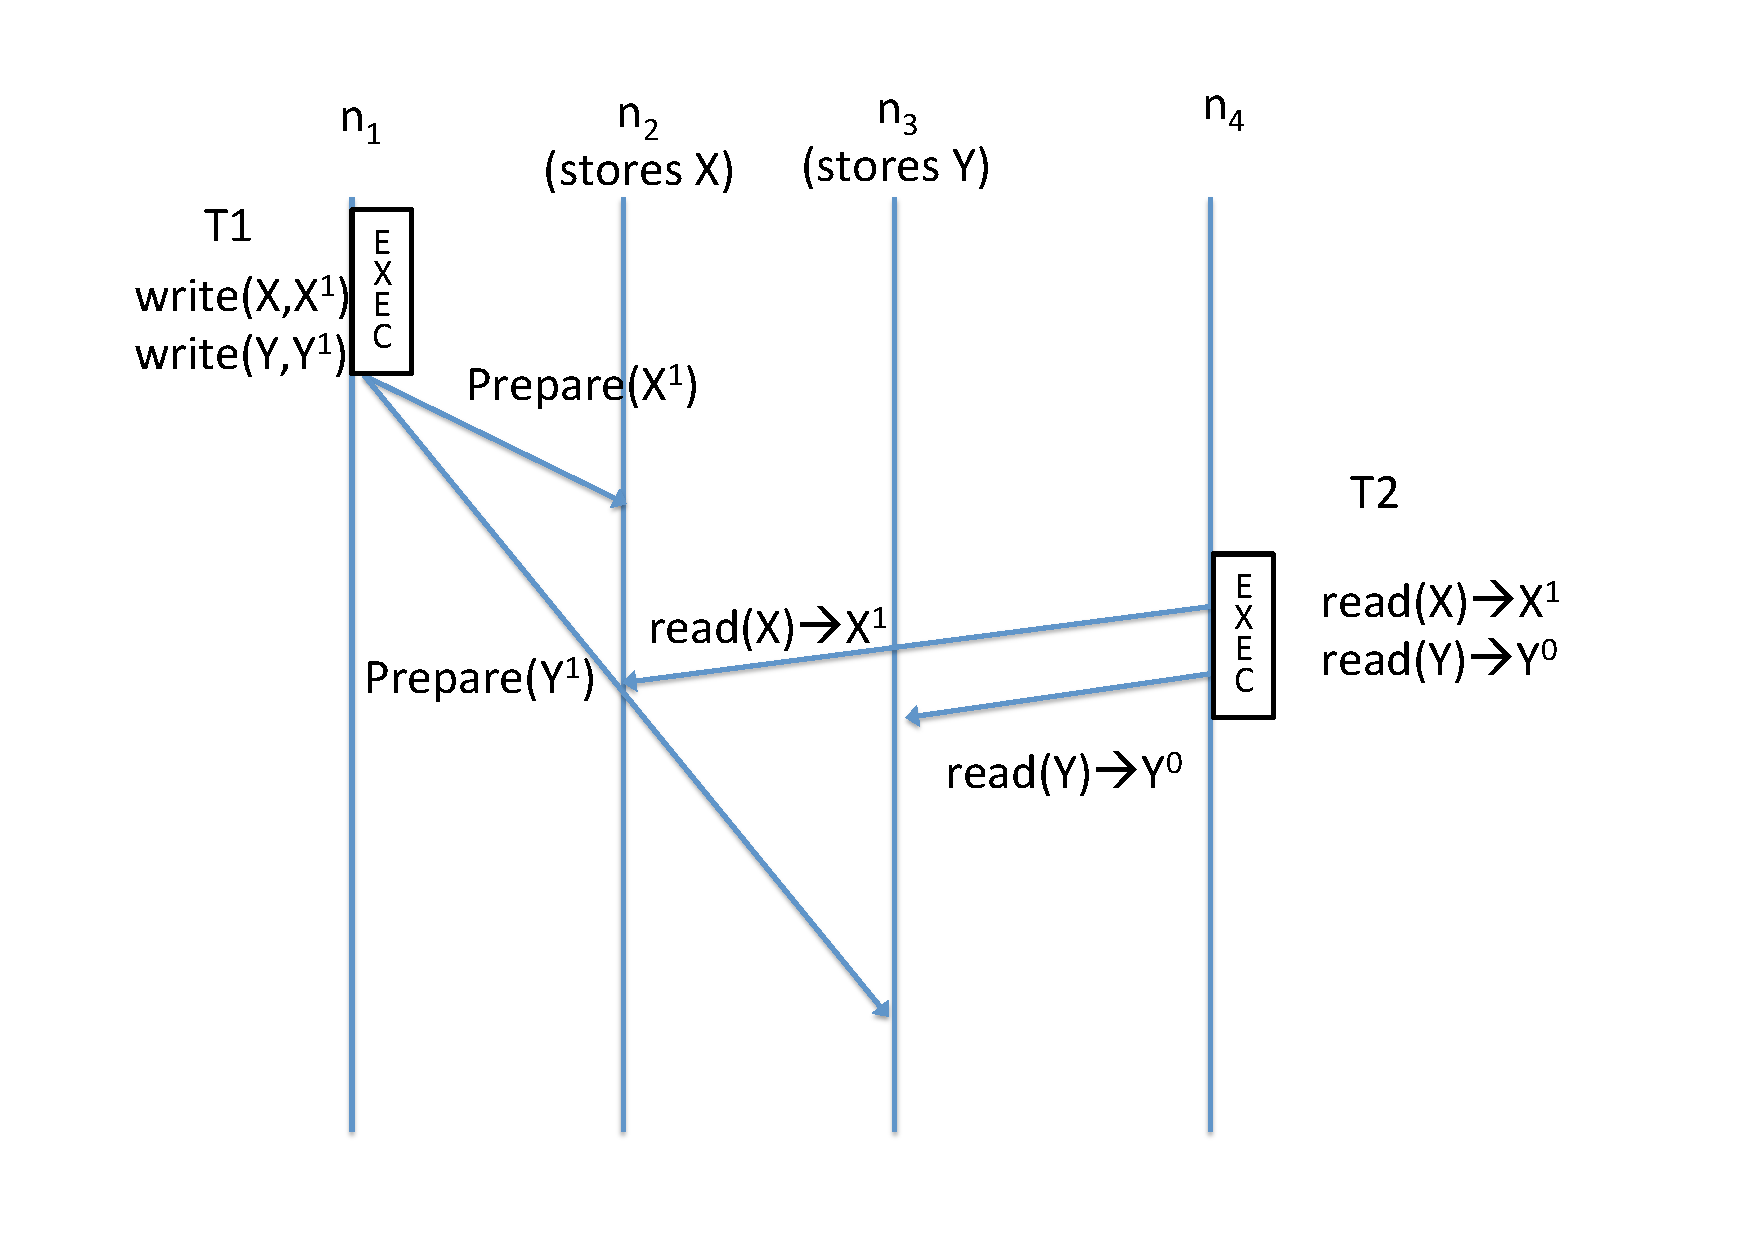
\includegraphics[scale = 0.24]{figures/example1.pdf}
%\caption{\footnotesize Atomicity violation --- T2 observes partially the updates of T1 (on data item X, but not on Y).}
%\label{fig:ex1}
%\end{minipage}\\
%\begin{minipage}{.48\textwidth}
%\hspace{-5mm}
%\centering
%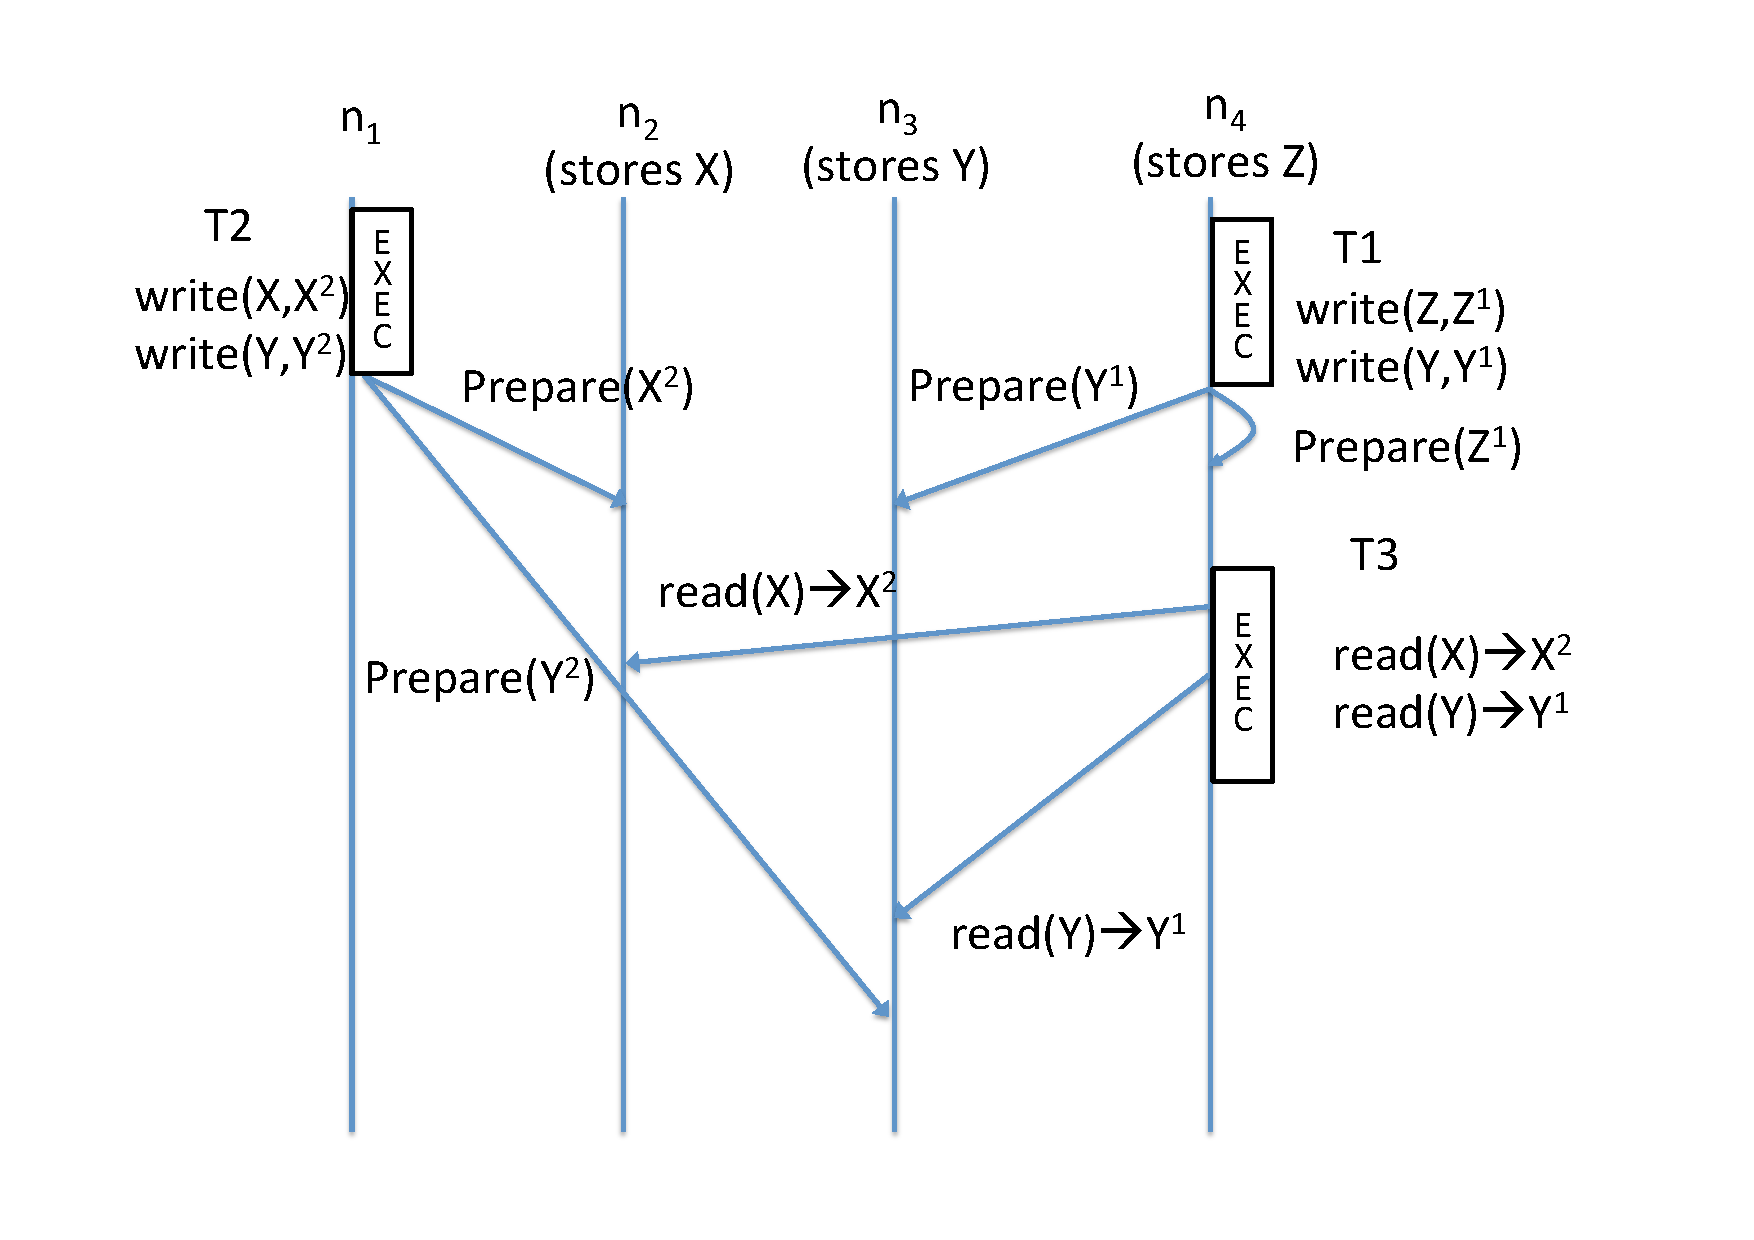
\includegraphics[scale = 0.24]{figures/example2.pdf}
%\caption{\footnotesize Isolation violation --- T3 observes the updates of two conflicting transactions, namely T1 and T2.}
%\label{fig:ex2}
%\end{minipage}
%\caption{\footnotesize Examples of concurrency anomalies that may arise when adopting speculative techniques that are prevented by the SPSI criterion.}
%\label{fig:example}
%\end{figure}

\begin{figure}[t!]
\centering
\hspace{-5mm}
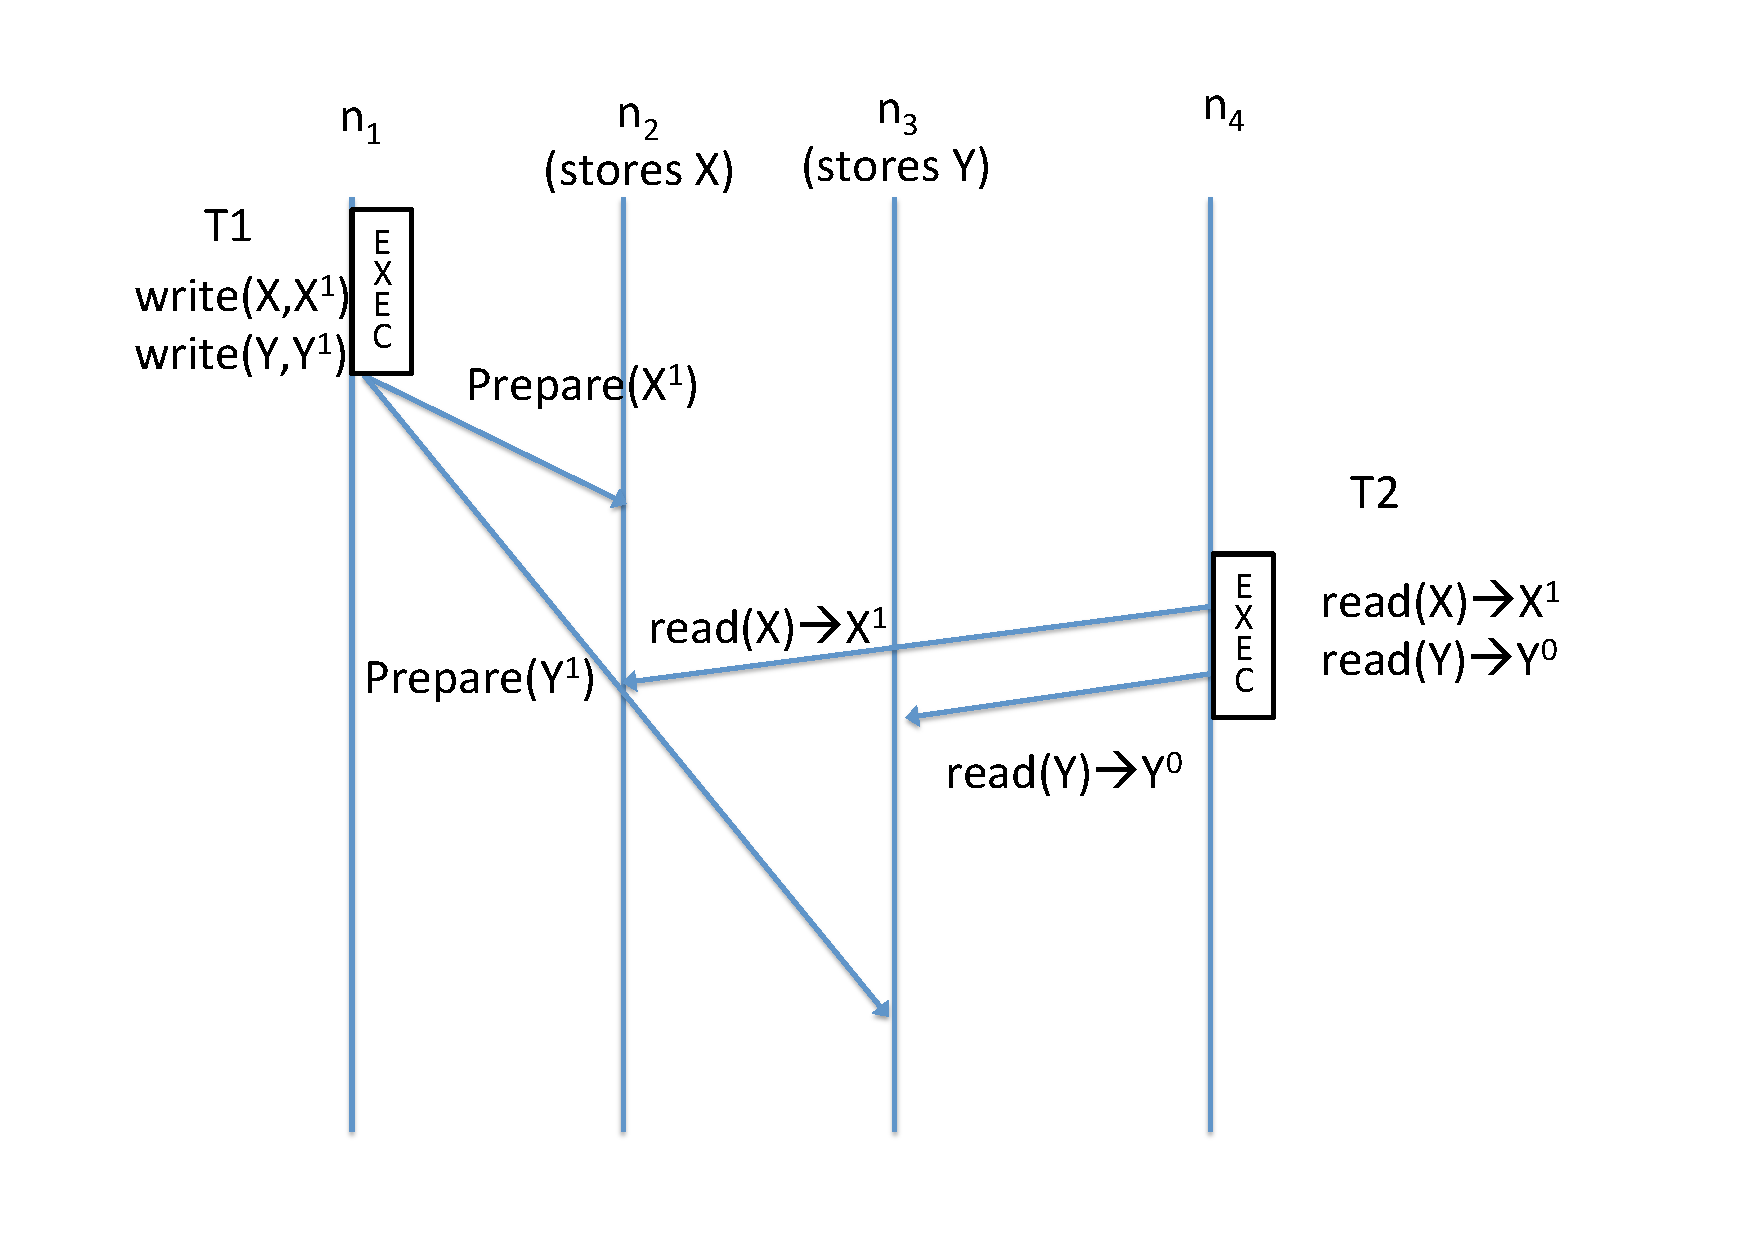
\includegraphics[scale = 0.24]{figures/example1.pdf}
\vspace{-5mm}
\caption{\footnotesize Atomicity violation --- T2 observes partially the updates of T1 (on data item X, but not on Y).}
\label{fig:ex1}
\vspace{-5mm}
\end{figure}

\begin{figure}[t!]
\centering
\hspace{-5mm}
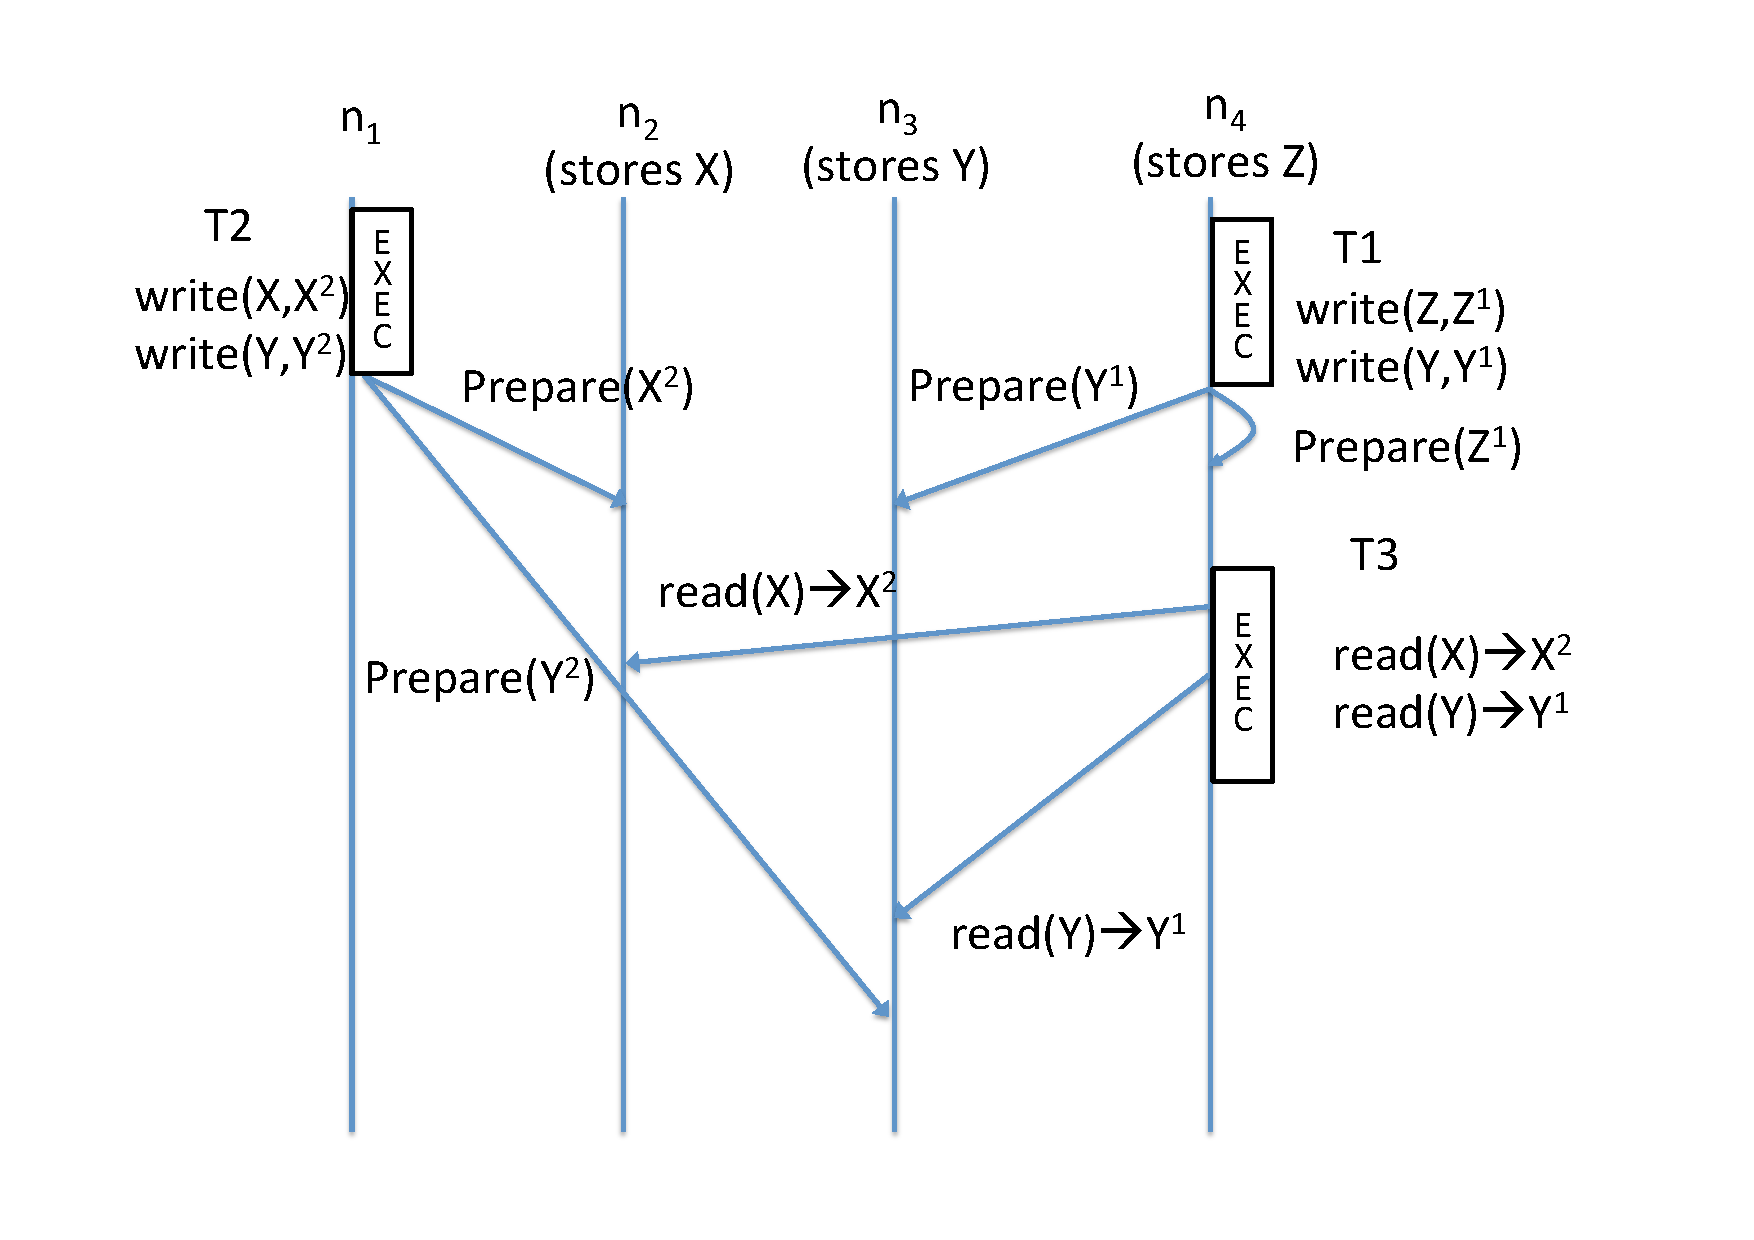
\includegraphics[scale = 0.24]{figures/example2.pdf}
\vspace{-5mm}
\caption{\footnotesize Isolation violation --- T3 observes the updates of two conflicting transactions, namely T1 and T2.}
\label{fig:ex2}
\vspace{-5mm}
\end{figure}

Figures~\ref{fig:ex1} and~\ref{fig:ex2} illustrate two examples of concurrency anomalies that can arise in a transactional system that adopts speculative reads. In Figure~\ref{fig:ex1}, the atomicity of transaction T1 is violated, as transaction T2 observes only partially T1's updates, i.e., it speculatively reads the version of X produced by T1 but misses T1's updates on Y. Figure~\ref{fig:ex2} illustrates a violation of the isolation properties ensured by SI, since T3 reads speculatively the versions of data items X and Y  produced by two transactions, i.e., T1 and T2, which conflict on X and cannot, hence, be both committed. This type of anomalies can be quite hard to predict or reason about, as they can manifest as subtle concurrency bugs that can lead to anomalous system states, e.g., divisions by zero or infinite cycles~\cite{guerraoui2007opacity}, and compromise the safety of user level applications, e.g., by crashing them.

\vspace{4pt}\noindent {\bf Performance robustness.} If used injudiciously, speculation can actually hamper, instead of benefiting performance. As we will show, in adverse scenarios  --- e.g., large likelihood of transaction aborts and high system load --- the additional costs associated with mispeculations can significantly penalize both user perceived latency and the maximum throughput achievable by the system.

Further, in order to maximize the benefits attainable in favourable workload settings, it is essential that the mechanisms employed to support speculation are very lightweight and efficient. Else, the overheads they impose may shadow or even outweigh the performance gains effectively achievable using speculative techniques.


We tackle the first of the above challenges by introducing a novel consistency model, which we termed Speculative Snapshot Isolation (SPSI). SPSI extends the classic Snapshot  Isolation (SI) criterion in order to provide clear and stringent guarantees on the atomicity and isolation of the snapshots observed and produced in execution histories to encompass both speculative reads and speculative commits.  %SPSI is designed to prevent the concurrency anomalies illustrated by the example in Figure~\ref{fig:example} {\bf TODO: add second example with isolation violation} while preserving the simplicity and intuitiveness of SI.  %with the ultimate goal of masking away complexity from .

% Figure~\ref{fig:example} illustrates one of possible concurrency anomalies that can arise in a transactional system that adopts weak consistency, by exposing the data item versions produced by speculatively committed transactions: transaction T3 observes the version of data item X precommitted by a concurrent transaction, T2, on node n$_1$. However, when it comes to reading Y, which was also updated by T2, T3 misses the version created by T2 on node n$_3$ (as T2's updates are still being propagated to node \textit{n$_2$}).
 
In a nutshell, SPSI guarantees that the snapshots that can be observed/speculatively committed by a transaction T originated at a node \textit{n}
 are equivalent to the ones that T would have observed/committed, had it been executed by a non-speculative SI data store along with all the transactions existing in the system, with the exception of any speculatively committed transaction originated at a different node $n'\neq n$. Unlike SI, though, SPSI allows a transaction T to include, in its snapshot to observe, the data item versions produced by transactions that speculatively committed before T started.
 
SPSI  spares programmers from complex concurrency bugs, by ensuring that  transactions always execute on snapshots that are atomic and isolated, although not capturing the effects of concurrent, speculatively committed remote transactions. Further, by demanding that the snapshots over which transactions execute reflect \textit{only} the effects of locally activated concurrent transactions, SPSI's specification allows for efficient implementations that can decide whether it is safe to speculatively commit a transaction solely on the basis of local information.


SPSI represents the theoretical foundations over which we build \specula (Speculative Transactional Replication). The protocol employed by \specula  shares several key design choices with state-of-the-art strongly consistent data stores~\cite{spanner,clocksi,peluso2012score}, which contribute to its efficiency and scalability. These include:  multi-versioning, which maximizes efficiency in read-dominated workloads~\cite{bernstein1987concurrency},  purely decentralized concurrency control based on distributed clocks~\cite{spanner,clocksi,peluso2012scalability}, as well as support for partial replication. 

However, unlike conventional transactional protocols, \specula supports both 
the speculative read and speculative commit mechanisms. As we will show via an extensive experimental study, \specula's design choice of allowing speculative read can lead to increase throughput by up to XX$\times$ and reduce latency by up to YY$\times$. Such gains can be achieved in a fully transparent way for programmers, allowing applications designed to run on a SI-compliant data store to run unmodified on \specula.

Applications that exploit \specula's speculative commit mechanism can reduce the client-perceived latency by up to an additional XX\% factor. By reducing the execution latency of transactions,  speculative commits also allow for enhancing the throughput achievable by \specula by up to XX$\times$ in machine-to-machine applications in which the rate of submission of new transactions is solely throttled by the speed at which the system can process previously submitted transactions. As the usage of speculative commits allow mispeculations to surface and be exposed to clients, applications that use this mechanism do have to be equipped with compensation logic to handle scenarios in which speculatively committed transactions' have to be eventually aborted.  Yet, \specula's programming model allows developers to use speculative commits selectively, i.e., on a subset of the application's transactions. This allows programmers to extend their applications, in an incremental and modular fashion, and/or to focus only on  transactions that have a critical impact on user-perceived latency.

Finally, in order to achieve performance robustness, \specula integrates a lightweight, yet effective, hill climbing-based self-tuning  mechanism that dynamically adjusts the aggressiveness of the speculative mechanisms employed by the system based on the workload characteristics. Not only self-tuning allows \specula to remain competitive in challenging scenarios that are unfavourable to the use of speculative techniques. It also allows to automatically identify which configurations maximize the performance gains achievable via speculation in favourable workloads, sparing the complexity of manually tuning any additional system's knobs.

The remainder of this paper is structured as follows. {\bf TODO}


